\section{Conductors and Circuits}
We're going to start talking about things behave when they interact with electric charges, and in general, we classify objects as conductors or insulators based on the ability for charged particles to be transferred across it. For example, insulators like glass and rubber, when charged, don't leak charge to their environment, whereas conductors like metals will, for lack of a better term, conduct charge so that it is spread evenly. When no net charge is flowing from place to place, we say that the conductor has reached electrostatic equilibrium. In this case, the electric field inside the conductor is zero. (This does NOT mean that the potential inside is zero, but rather, is constant - we'll see an example of this). 
\subsection{Ohmic Conductors}
When a potential difference is created across a conductor, electrostatic equilibrium is disrupted and an electric field is created inside the conductor. This causes the flow of charge carriers (electrons) through the conductor, and this flow of charge is called current, usually denoted with an uppercase or lowercase $I$. (I will use the uppercase $I$, because I don't want it to be confused with the imaginary unit.) Current has units of coulombs per second, also called an ampere (A). We also use current density $j$ (a vector quantity), which relates to how the current flows through some cross-sectional area of the solid, and has units of ampere per square meter. The current density vector describes how much current flows through that point inside the solid, and in what direction it flows. The flux of the current density through a surface is the current through that surface - put quantitatively,
\[
	dI = \vec j \cdot \hat n \, dA
\] 
Of course, for non-uniform surfaces, this becomes a surface integral, where you cut up the curved surface into small areas and calculate the current through each area: 
\[
	I = \int_S \vec j \cdot \hat n \, dA
\]
Let's discuss some other properties of the current density. For a conductor of uniform cross section $A$, which has a current flowing through it with uniform current density $j$, we can imagine the current pushing charged particles along at a speed of $v_d$. This is the drift speed of electrons inside the conductor. Notice that we are basically using a fluid to model the flow of charge, like that of water - which is remarkably the truth! Electrons are an incompressible fluid, and don't do weird things like build up in places where they shouldn't - the displacement of one charged particle leads to all of the charge being displaced, which is pretty easy to model.\\
\begin{center}
	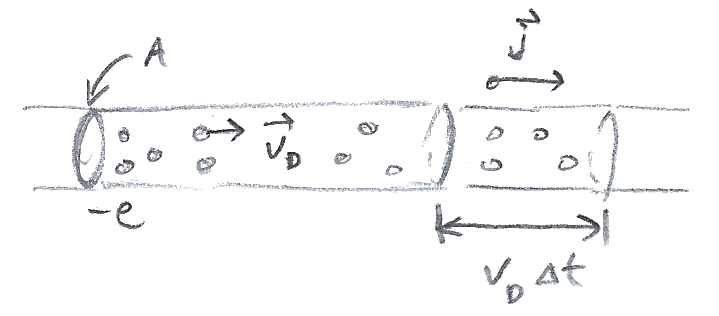
\includegraphics[scale=0.4]{images/em/playdoh.png}\\
\end{center}
In a time $\Delta t$, the volume of the charged particles displaced is $Av_d \Delta t$. The charge pushed through is then the volume times the charge density per unit volume $\rho$. On the other hand, we can express the charge pushed through directly in terms of the current $I = jA$. The charge moved in a time $\Delta t$ is just $I\Delta t = jA \Delta t$. We can equate this and get:
\[
	Av_d\Delta t \rho = jA\Delta t \rightarrow 	v_d \rho = j 
\]
Sometimes we will also see $n$, the number density of charged particles per cubic meter, and usually, we'll see electrons flowing, so we'll see the charge $e$ as well in this equation. Notice that in terms of magnitude, we have $\rho = en$, so 
\[
	j = v_d en
\]
We can also express this in vector form: it is also true that 
\[
	\vec j = -en \vec v_d
\]
We have to be careful, however - if the charges of the particles are negative, as is the case for electrons, then the drift velocity of the electrons are in the opposite direction as the current. Therefore, it's from this that I have to warn you - even though we may know the direction of the current in a wire, without other information we can't tell whether or not the current consists of positively-charged particles moving in the direction of the current or negatively-charged particles moving opposite to it. \\
It turns out that the current density is also directly related to the electric field for some conductors, through a relation called Ohm's Law. This isn't the regular form of Ohm's Law that you're used to, it's the differential form - but we'll see how to get there from the differential form. \\
Ohm's Law (differential form) states that 
\[
	\vec j = \sigma \vec E
\]
In this case, $\sigma$ is not the charge density, it's the proportionality constant called the conductivity of the material. Conductors that follow this rule are called ohmic conductors, and a large number of conductors follow this rule (not in extreme cases). \\
\begin{center}
	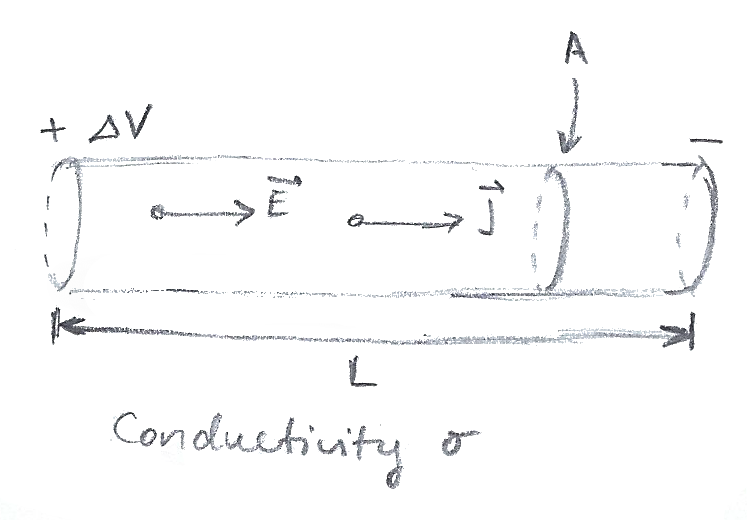
\includegraphics[width=0.4\textwidth]{images/em/ohmic-conductor.png}\\
\end{center}
For simplicity, let's assume we have a conductor with length $L$ and uniform cross section $A$, and that this electric field $E$ is created from exerting a constant potential difference $\Delta V$ across the ends of the conductor. Let's also just consider the magnitudes of the current density and electric field and multiply through on both sides by the volume of the conductor, $LA$:
\[
	L A j = \sigma E L A
\]
We can group the terms in certain ways to get the potential difference $\Delta V$ and the current $I$. Namely, the potential difference $\Delta V = EL$, and the current $I = jA$, so substituting we have:
\[
	LI = \sigma A \Delta V
\]
We can now isolate $\Delta V$:
\[
	\Delta V = I \frac{L}{A\sigma} = IR
\]
This fractional term that appears is defined as the resistance $R$ of the object. Resistance, as you may know, is measured in ohms ($\Omega$).  For the cases we will consider on a regular basis, this is sufficient. Sometimes it's written like this:
\[
	R = \frac{L}{A}\rho
\]
where $\rho = \frac{1}{\sigma}$ is the resistivity of the object. This, along with the above, gives us enough relations to be able to calculate most properties of a conductor given some information. 
\subsection{Capacitance}
Capacitance is a property of conductors that indicates the ability to store charge due to a potential difference. If two separated conductors are charged to $+Q$ and $-Q$, respectively, by a potential difference of $V$, then the capacitance $C$ of this system is given by 
\[
	C = \frac{Q}{V}
\]
This system of two conductors is called a capacitor, and the capacitance of a capacitor is measured in farads (F), named after Michael Faraday. It turns out the capacitance of a capacitor is dependent only upon the geometry of the system and the permittivity of free space $\epsilon_0$ (unless there's a material that's not air between the two conductors, which we will discuss later). This seems unlikely - but we can show that this is true intuitively. \\
Consider that on the surface of these two conductors the magnitude of the charge of each of them is doubled. Therefore, since the electric field generated by the conductors is proportional to the charge of the source of the field, therefore the electric field must be doubled. Because of this, the potential difference between the two capacitors also doubles, and since the potential difference and charge scale up by the same amount when the charge changes, the ratio between them remains constant. So, the capacitance remains constant independent of the charge of the conductors, so it must be dependent on the configuration of the system (geometrically) and the permittivity $\epsilon_0$. One can see that the unit for a farad and the units of $\epsilon_0$ differ by a factor of a meter, and one can often write $\epsilon_0$ as 8.854 $\cdot$ 10$^{-12}$ F/m, as it's the cleanest way to write the units. \\
In order to charge the capacitor, energy clearly needs to be input in order to move charge from one conductor to the other in order to create this imbalance. We can calculate the total energy required to move a total charge $Q$ from one conductor to the other. For a small charge $dq$, the amount of work needed to move against the potential difference $V(q) = \frac{q}{C}$ is 
\[
	dW = V(q) \, dq = \frac{q}{C} \, dq
\]
We can integrate from $0$ to $Q$: 
\begin{align*}
	W &= \int_0^Q \frac{q}{C} \, dq \\
	&= \frac{1}{2} \frac{q^2}{C} \Big|_0^Q\\
	&= \frac{1}{2} \frac{Q^2}{C} = \frac{1}{2}QV = \frac{1}{2}CV^2
\end{align*}
This energy is stored in the capacitor as potential energy, and in fact, it's stored in the electric field generated by this imbalance of charge. The electric field has an energy density per unit volume within it - it turns out that this energy density $u = \frac{1}{2}E^2 \epsilon_0$, but knowing how this formula is derived is beyond the scope of this course.\\
The most common capacitor we will encounter is the parallel-plate capacitor. It's two squares of charge with area $A$ and surface charge density $\sigma$, and whose plates are separated by a distance $d$.
\begin{center}
	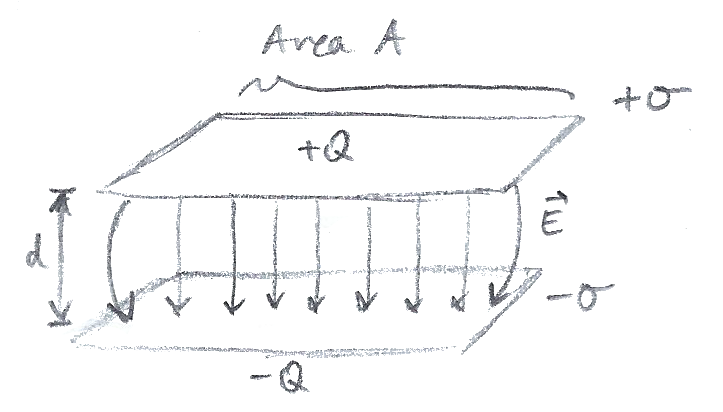
\includegraphics[width=0.4\textwidth]{images/em/capacitor.png}
\end{center}
From electrostatics, since each plane contributes a field of $\frac{\sigma}{2\epsilon_0}$ to the electric field, the total electric field is $\frac{\sigma}{\epsilon_0}$. (These fields don't cancel each other out as the field lines point the same direction). We can effectively consider the plates as planes of charge, even though they are finite. Only at the edges of the capacitor does the electric field become non-uniform, so approximately speaking, far from the edges of the planes, this is true. Even with this in mind, we can derive the potential difference as $V = \frac{\sigma d}{\epsilon_0}$. The charge on each capacitor plate is $Q = \sigma A$, so then the capacitance $C$ is:
\[
	C = \frac{Q}{V} = \frac{\sigma A}{\frac{\sigma d}{\epsilon_0}} = \frac{A \epsilon_0}{d}
\]
The energy stored in the field of the capacitor can then be found to be:
\[
	U = \frac{1}{2}QV = \frac{1}{2} \sigma A \frac{\sigma d}{\epsilon_0} = \frac{\sigma^2 Ad}{2\epsilon_0}
\]
The density of this field, according to our formula, is:
\[
	u = \frac{1}{2} \epsilon_0 \left(\frac{\sigma}{\epsilon_0}\right)^2 = \frac{\sigma^2}{2\epsilon_0}
\]
And observe that if we multiply through by the volume, $Ad$, the correct expression for the energy stored appears, confirming the consistency of the energy density formula for this particular case (which is still true in general). \\
We can now discuss the more complicated case if something is inserted between the two conductors. In this case, the insertion of some solid increases the permittivity in the object by a scalar $\kappa$, called the dielectric constant. The new object's permittivity $\epsilon = \kappa \epsilon_0$. This, in turn, increases the capacitance of the capacitor by the same constant $\kappa$, so the new capacitance $C_f$ as compared to the original, $C_i$, is:
\[
	C_f = \kappa C_i
\]
Simple enough. Usually this constant is obtained by measurement, so the dielectric constant will be given most of the time. Since a dielectric changes the permittivity of the space between the plates from $\epsilon_0$ to $\epsilon = \kappa \epsilon_0$, this means that the electric field weakens by a factor of $\kappa$ inside the dielectric material. Charges are induced on the surface of the dielectric of the opposite sign as the charge on the closer plate, because the charges on the capacitor plates polarize the material. Note that the combined charges on the capacitor plate and on the surface of the dielectric should produce the total electric field in the material. Since the electric field strength decreases by a factor of $\frac{1}{\kappa}$, the total charge of the plate and the dielectric is $\frac{1}{\kappa}$ times the original and therefore the charges induced on the surface of the dielectric must have magnitude  $1 - \frac{1}{\kappa}$ and of the opposite sign in order to align with this. \\
As far as capacitors go, they store energy in an electric field. We'll soon see their behavior in circuits, where they will be a complication to the resistor-only circuits seen in Design and Tech. 
\subsection{Circuits and Kirchhoff's Laws}
The culmination of talking about conductors and their properties is their application in building and analyzing circuits. In a closed circuit, there is always some way where a potential difference $V$ is exerted on the wire that allows electrons to travel through it, creating a current. The most common way this is done is by a constant source of electrical energy, like a battery, that produces an electromotive force (emf) $\mathscr{E}$. In a circuit, the main circuit component that provides resistance are resistors, and the main component that provides capacitance to the circuit is the capacitor, as discussed earlier. We will later discuss a quantity called inductance and another circuit element, inductors, but not until we talk about magnetism. \\
A short digression on batteries - as you might remember from chemistry, batteries are powered by a redox reaction that creates a potential difference between the two electrodes of the battery. As electrons pass from the negatively charged electrode to the positively charged electrode, the anode (-) becomes more and more negatively charged, and the cathode (+) becomes more and more positively charged. Eventually, the negative ions will be depleted and therefore the battery will decrease in its potential until it reaches 0. Ideally, however, we will deviate from reality and assume our batteries will maintain a constant emf $\mathscr{E}$. Furthermore, since everything has some internal resistance, we sometimes might add a small resistor $r$ to a circuit to model this internal resistance. \\
Another assumption that we make regarding a circuit is that the conductor through which electrons flow, the wire, has negligible internal resistance. Of course, this is not true because we can calculate it using ideas from our analysis of conductors and their properties, but we will omit it when discussing circuits. \\
The most important rules that we can use to analyze circuits is Kirchhoff's Loop Rules. There are only two:\\
Kirchhoff's Voltage Law (KVL):  Around a closed loop, the sum of the potential differences is zero. \\
Kirchhoff's Current Law (KCL): At a junction in a circuit, the total current going in is equal to the total current going out. \\
These can be derived from principles we already know. For KVL, recall that because the electric force is conservative, we have that the line integral of the force on a charged particle around a closed loop is zero. Considering this expression per unit charge, we have:
\[
	\oint_C \vec F \cdot \, d\vec s = 0 \rightarrow \oint_C \vec E \cdot \, d\vec s = 0
\]
However, this is the same as looking at the potential around a closed loop, so this too is zero. For KCL, we can notice that because charge is conserved, all of the charge that flows into a junction must flow out. \\
We can use these rules to look at capacitors and resistors in series and parallel before moving to analyze our first (time-dependent!) circuit. As a reminder, "series" refers to on the same branch, while "parallel" refers to on different branches. \\
First, we can take a look at these circuit components in parallel. (Our derivations here can be extended to more than two capacitors/resistors.)\\
For two capacitors in parallel with capacitances $C_1$ and $C_2$, and a voltage $V$ across the system, we can try to calculate the total capacitance of the system. Assume that the charge on each of these capacitors, when fully charged, are $Q_1$ and $Q_2$, respectively. The capacitance of a capacitor $C$ that would have the same capacitance as these two capacitors in parallel would be:
\[
	C = \frac {Q^{tot}}{V}
\]
Notice that $Q^{tot} = Q_1 + Q_2$ by conservation of charge. We can then split this:
\[
	C = \frac{Q_1}{V} + \frac{Q_2}{V}
\]
As the voltage across each branch is the same as the voltage across the system, we have that:
\[
	C = \frac{Q_1}{V_1} + \frac{Q_2}{V_2} = C_1 + C_2
\]
We can do a similar analysis for resistors. For two resistors in parallel with resistances $R_1$ and $R_2$, and currents $I_1$ and $I_2$ across each resistor, we can look at the total resistance $R$ in terms of Ohm's Law:
\[
	R = \frac{V}{I}
\]
where $I$ is the total current going into/out of the branches. By Kirchhoff's Current Law, $I = I_1 + I_2$, and so we can make this substitution:
\[
	R = \frac{V}{I_1 + I_2} = \frac{1}{\frac{I_1+I_2}{V}}
\]
We can re-apply Ohm's Law on the denominator:
\[
	R = \frac{1}{\frac{I_1}{V} + \frac{I_2}{V}} = \frac{1}{\frac{I_1}{V_1} + \frac{I_2}{V_2}} = \frac{1}{\frac{1}{R_1} + \frac{1}{R_2}}
\]
Rearranging, we have:
\[
	\frac{1}{R} = \frac{1}{R_1} + \frac{1}{R_2}
\]
We can repeat this for capacitors and resistors in series. For a system of two capacitors with capacitances $C_1$ and $C_2$, and a voltage $V$, we can imagine a capacitor with capacitance $C$ equal to the total capacitance of both capacitors. The voltage drop for each capacitor $V_1$ and $V_2$ sum to the total voltage $V$, so $V_1 + V_2 = V$. The charge on each capacitor $Q_1$ and $Q_2$ are both equal to the total charge through the system $Q$ since the current is the same going through both capacitors. We can calculate the capacitance now:
\[
	C = \frac{Q}{V} = \frac{Q}{V_1+V_2} = \frac{1}{\frac{V_1+V_2}{Q}} = \frac{1}{\frac{V_1}{Q} + \frac{V_2}{Q}} = \frac{1}{\frac{V_1}{Q_1} + \frac{V_2}{Q_2}} = \frac{1}{\frac{1}{C_1} + \frac{1}{C_2}}  
\]
The most compact way to write this is:
\[
	\frac{1}{C} = \frac{1}{C_1} + \frac{1}{C_2}
\]
For two resistors $R_1$ and $R_2$ with current $I_1$ and $I_2$ across them, we can find the total resistance $R$ using Ohm's Law, noting that the total current $I = I_1 = I_2$:
\[
	R = \frac{V}{I} = \frac{V_1 + V_2}{I} = \frac{V_1}{I} + \frac{V_2}{I} = \frac{V_1}{I_1} +  \frac{V_2}{I_2} = R_1 + R_2
\]
With these relations to condense resistors/capacitors in series and in parallel, we can now always effectively condense circuits to one resistor and one capacitor. Let's analyze the simplest 1-loop circuit with a resistor and a capacitor - the simplest RC circuit.
\begin{center}
	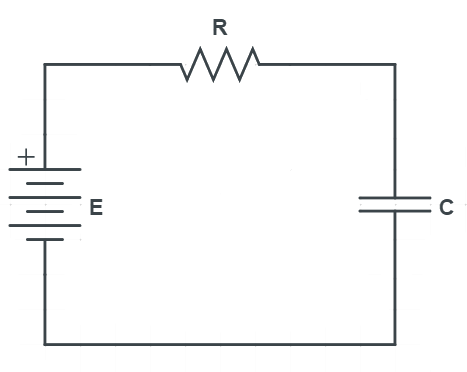
\includegraphics[scale=0.25]{images/em/RC-circuit.png}
\end{center}
Consider a battery with emf $\mathscr{E}$, a resistor with resistance $R$, and a capacitor with capacitance $C$. Let $Q$ denote the charge on the capacitor as a function of time and $I$ the current. When the switch is initially flipped to complete the circuit, assume no charge lies on the plates of the capacitor. From KVL, we have, at any given moment:
\[
    \mathscr{E} - IR - \frac{Q}{C} = 0
\]
Noting that $I = \frac{dQ}{dt}$, we can rewrite this as our first first-order differential equation:
\[
    \mathscr{E} - R\dv{Q}{t} - \frac{Q}{C} = 0 
\]
\[
    R\dv{Q}{t} =  \frac{\mathscr{E}C - Q}{C}  
\]
\[
    \frac{RC}{\mathscr{E}C-Q}\dv{Q}{t} = 1
\]
Integrating from time $t=0$ to arbitrary time $t$, we have:
\[
    \int_0^t\frac{RC}{\mathscr{E}C-Q}\dv{Q}{t}\, dt = \int_0^t 1 \, dt
\]
\[
    -RC \ln\left(\frac{\mathscr{E}C-Q(t)}{\mathscr{E}C}\right) = t
\]
\[
    \mathscr{E}C-Q(t) = \mathscr{E}Ce^{-\frac{t}{RC}}
\]
\[
    Q(t) = \mathscr{E}C\left(1-e^{-\frac{t}{RC}}\right)
\]
We can take the derivative to find the current $I$:
\[
	I = \dv{Q}{t} = \dv{}{t} \mathscr{E}C\left(1-e^{-\frac{t}{RC}}\right) = \frac{\mathscr{E}}{R}e^{-\frac{t}{RC}}
\]
When the circuit is closed at time $t=0$, the current $I = \frac{\mathscr{E}}{R}$, which is basically the same as if there was no capacitor and instead just a wire. In general, at the beginning of the charging of a capacitor, the capacitor acts like a wire. As $t \to \infty$ and approaches the steady state, the charge on the capacitor approaches $\mathscr{E} C$, and the current approaches zero. This is because the energy from the voltage that the capacitor extracts from the circuit is stored into the electric field of the capacitor, and eventually this will force the current to decrease as to satisfy KVL. The resistor, on the other hand, extracts energy from the circuit and converts it into vibrations and heat energy that is released and not stored.\\
The time it takes for this process of charging the capacitor to occur is influenced by the magnitudes of $R$ and $C$.  In fact, RC circuits have a time constant $\tau = RC$ that serves as a measure of how fast/slow the circuit is charged. (Note: the time constant has units of seconds - in fact, an ohm-farad is a second. You can verify this by dimensional analysis.)\\
Sometimes we will be asked what the power through a component in a circuit is at a given moment. The power is simply the voltage difference across the component times the current flowing through it. If we are able to express the power as a function of time, we will be able to integrate it (hopefully) to find the energy dissipated/stored/released over a time interval, which is useful for keeping track where the energy goes in a circuit. 
\subsection{Summary and Problems}
This chapter covered a wide variety of topics, starting with the ability of conductors to conduct current, and identifying properties of conductors such as their conductivity, resistance, and capacitance. We also looked at our first circuits and looked at how to model the behavior of a circuit over time. Most of these problems will be either circuit problems (harder) or calculating a property of a conductor (easier).\\

\noindent\textbf{Problems:}\\
1. (1 $\bigstar$) Show the resistivity of a long straight wire of radius $r$ and length $L$ is $\frac{\Delta V\pi r^2}{IL}$, if $I$ is the current through the wire when a potential difference of $\Delta V$ is exerted across the ends of the wire.\\
2. (2 $\bigstar$) The electric field at point $P$ just outside the outer surface of a hollow spherical conductor of inner radius 10 cm and outer radius 20 cm has magnitude 455 N/C and is directed outward. When an unknown point charge Q is introduced into the center of the sphere, the electric field at P is still directed outward but is now 185 N/C. Show that the total charge on the inside surface of the shell is 1.20$\cdot$10$^{-9}$ C.\\
3. (1 $\bigstar$) The magnitude $J$ of the current density in a certain wire with a circular cross section of radius $R$ = 2.10 mm is given by $J$ = (4.00$\cdot$10$^8$)$r^2$, with $J$ in amperes per square meter and radial distance $r$ in meters. Show that the current through the outer section bounded by $r = 0.690R$ and $r = R$ is 9.45 mA.\\
4. (3 $\bigstar$) A metal ball with radius $R$ carries a total charge $Q$. The ball is surrounded by a thick conducting shell of inner radius $2R$ and outer radius $3R$. The total charge on the shell is zero and the conductors are in electrostatic equilibrium. Show that the electric potential of the metal ball relative to zero potential at infinity is $\frac{5kQ}{6R}$.\\
5. (4 $\bigstar$) A parallel plate capacitor of plate area $A$ and plate separation $d$ has a potential difference of $V_0$ is applied between the plates. Suppose that the battery remains connected while a dielectric slab of thickness $b$ and dielectric constant $\kappa$ is being introduced exactly between the two plates of the capacitor. Show that the electric field in the slab is $E = \frac{V_0}{\kappa d - (\kappa -1) b}$.\\
6. (3 $\bigstar$) The space between two concentric conducting spherical shells of radii $b$ and $a$ ($b>a$) is filled with a substance of dielectric constant $\kappa$. A potential difference $\Delta V$ is applied across the inner and outer shells. Show that the magnitude of the induced charge along the surface of the inner shell is $\frac{\Delta V 4\pi \epsilon_0 ab (\kappa -1)}{\kappa(b-a)}$.\\
7. (2 $\bigstar$) A charged isolated metal sphere of diameter $d$ has a potential $V$ relative to $V=0$ at infinity. Show that the energy density in the electric field near the surface of the sphere is $\frac{2V^2\epsilon_0}{d^2}$.\\
8. (2 $\bigstar$) A parallel-plate capacitor has plates of area $A$ and separation $d$ and is charged to a potential difference $V$. The charging battery is then disconnected, and the plates are pulled apart until their separation is $2d$. Show that the work required to pull these plates apart to this separation is $\frac{\epsilon_0AV^2}{2d}$.\\
9. (3 $\bigstar$, $\spadesuit$) A switch in an RC circuit is closed at time $t=0$, to begin charging an initially uncharged capacitor of capacitance $C$ through a resistor of resistance $R$. Show that in $RC \ln 2$ seconds, the voltage across the resistor will be the same as the voltage across the capacitor.\\
\begin{center}
	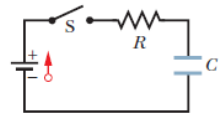
\includegraphics[scale=0.7]{images/em/RC-problem1.png}
\end{center}
10. (3 $\bigstar$) In the figure below, $R_s$ is to be adjusted in value by moving the sliding contact across it until points $a$ and $b$ are brought to the same potential. (One tests for this condition by momentarily connecting a sensitive ammeter between $a$ and $b$; if these points are at the same potential, the ammeter will not deflect.) Show that when this adjustment is made, we have that $R_x = \frac{R_sR_2}{R_1}$. \\
\begin{center}
	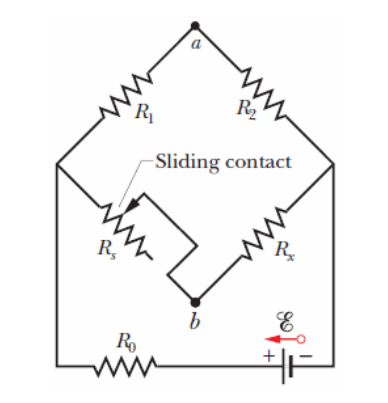
\includegraphics[scale=0.7]{images/em/circuit-problem1.png}
\end{center}
11. (2 $\bigstar$, $\spadesuit$) For the RC circuit shown in the figure below, the switch is initially closed to contact $a$. After having been at contact $a$ for a long time, the switch
throw is rotated to contact $b$. Once this happens, show that the charge on the capacitor can be modeled as a function of time as $Q(t) = \mathscr{E}Ce^{-t/RC}$.
\begin{center}
	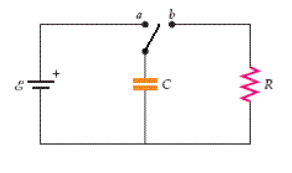
\includegraphics[scale=0.7]{images/em/RC-problem2.png}
\end{center}
12. (2 $\bigstar$) Using the same diagram at problem 11, show that the energy stored in the capacitor $U$ can be modeled as a function of time as $U(t) = \frac{1}{2}\mathscr{E}^2Ce^{-2t/RC}$.\\
13. (3 $\bigstar$) A cylindrical capacitor with an air gap has an inner radius of $r$, a thin outer shell with radius $R$, and length $L$. The capacitor is charged to a voltage difference of $\Delta V$. Show that the minimum energy density stored in the gap when the capacitor is fully charged is $\frac{1}{2} \epsilon_0 \left(\frac{\Delta V}{R\ln(r/R)} \right)^2$. \\
14. (3 $\bigstar$) Switch $S$, shown in the figure below, is closed after having been open for a long time. Show that the charges on the capacitors are 130 $\mu$C and 260 $\mu$C a long time after the switch has been closed. 
\begin{center}
	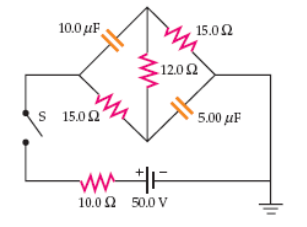
\includegraphics[scale=0.7]{images/em/RC-problem4.png}
\end{center}
\pagebreak